% pearltilus_annotated.tex -- TMA corner plot with mirror annotations and
% enlarged numbers. Overlays ../figures/pearltilus.png (panels: 200 px squares
% on a 210 px pitch, first panel at x=84, y=36 px). Parameter order in the
% image: pdx pdy pdz sdx sdy sdz ptx pty stx sty.
% The small corner titles and tick labels are covered and replaced by large
% parameter names and a summary table. Table values are the full-posterior
% medians and 16-84% intervals printed in the original corner titles
% (translations rounded to 1 um); axis spans are the prior ranges.
% Build: pdflatex pearltilus_annotated.tex
\documentclass[tikz,border=4pt]{standalone}
\usepackage[T1]{fontenc}
\usepackage[default]{sourcesanspro}
\usepackage{booktabs}
\usetikzlibrary{calc}
\definecolor{prim}{HTML}{4C78A8}
\definecolor{sec}{HTML}{F58518}
\definecolor{cross}{HTML}{B279A2}
\newlength\pxu
\setlength\pxu{0.013714cm}   % 2184 px -> 29.95 cm
\begin{document}
\begin{tikzpicture}[x=\pxu, y=\pxu]
  \node[anchor=south west, inner sep=0pt] at (0,0)
    {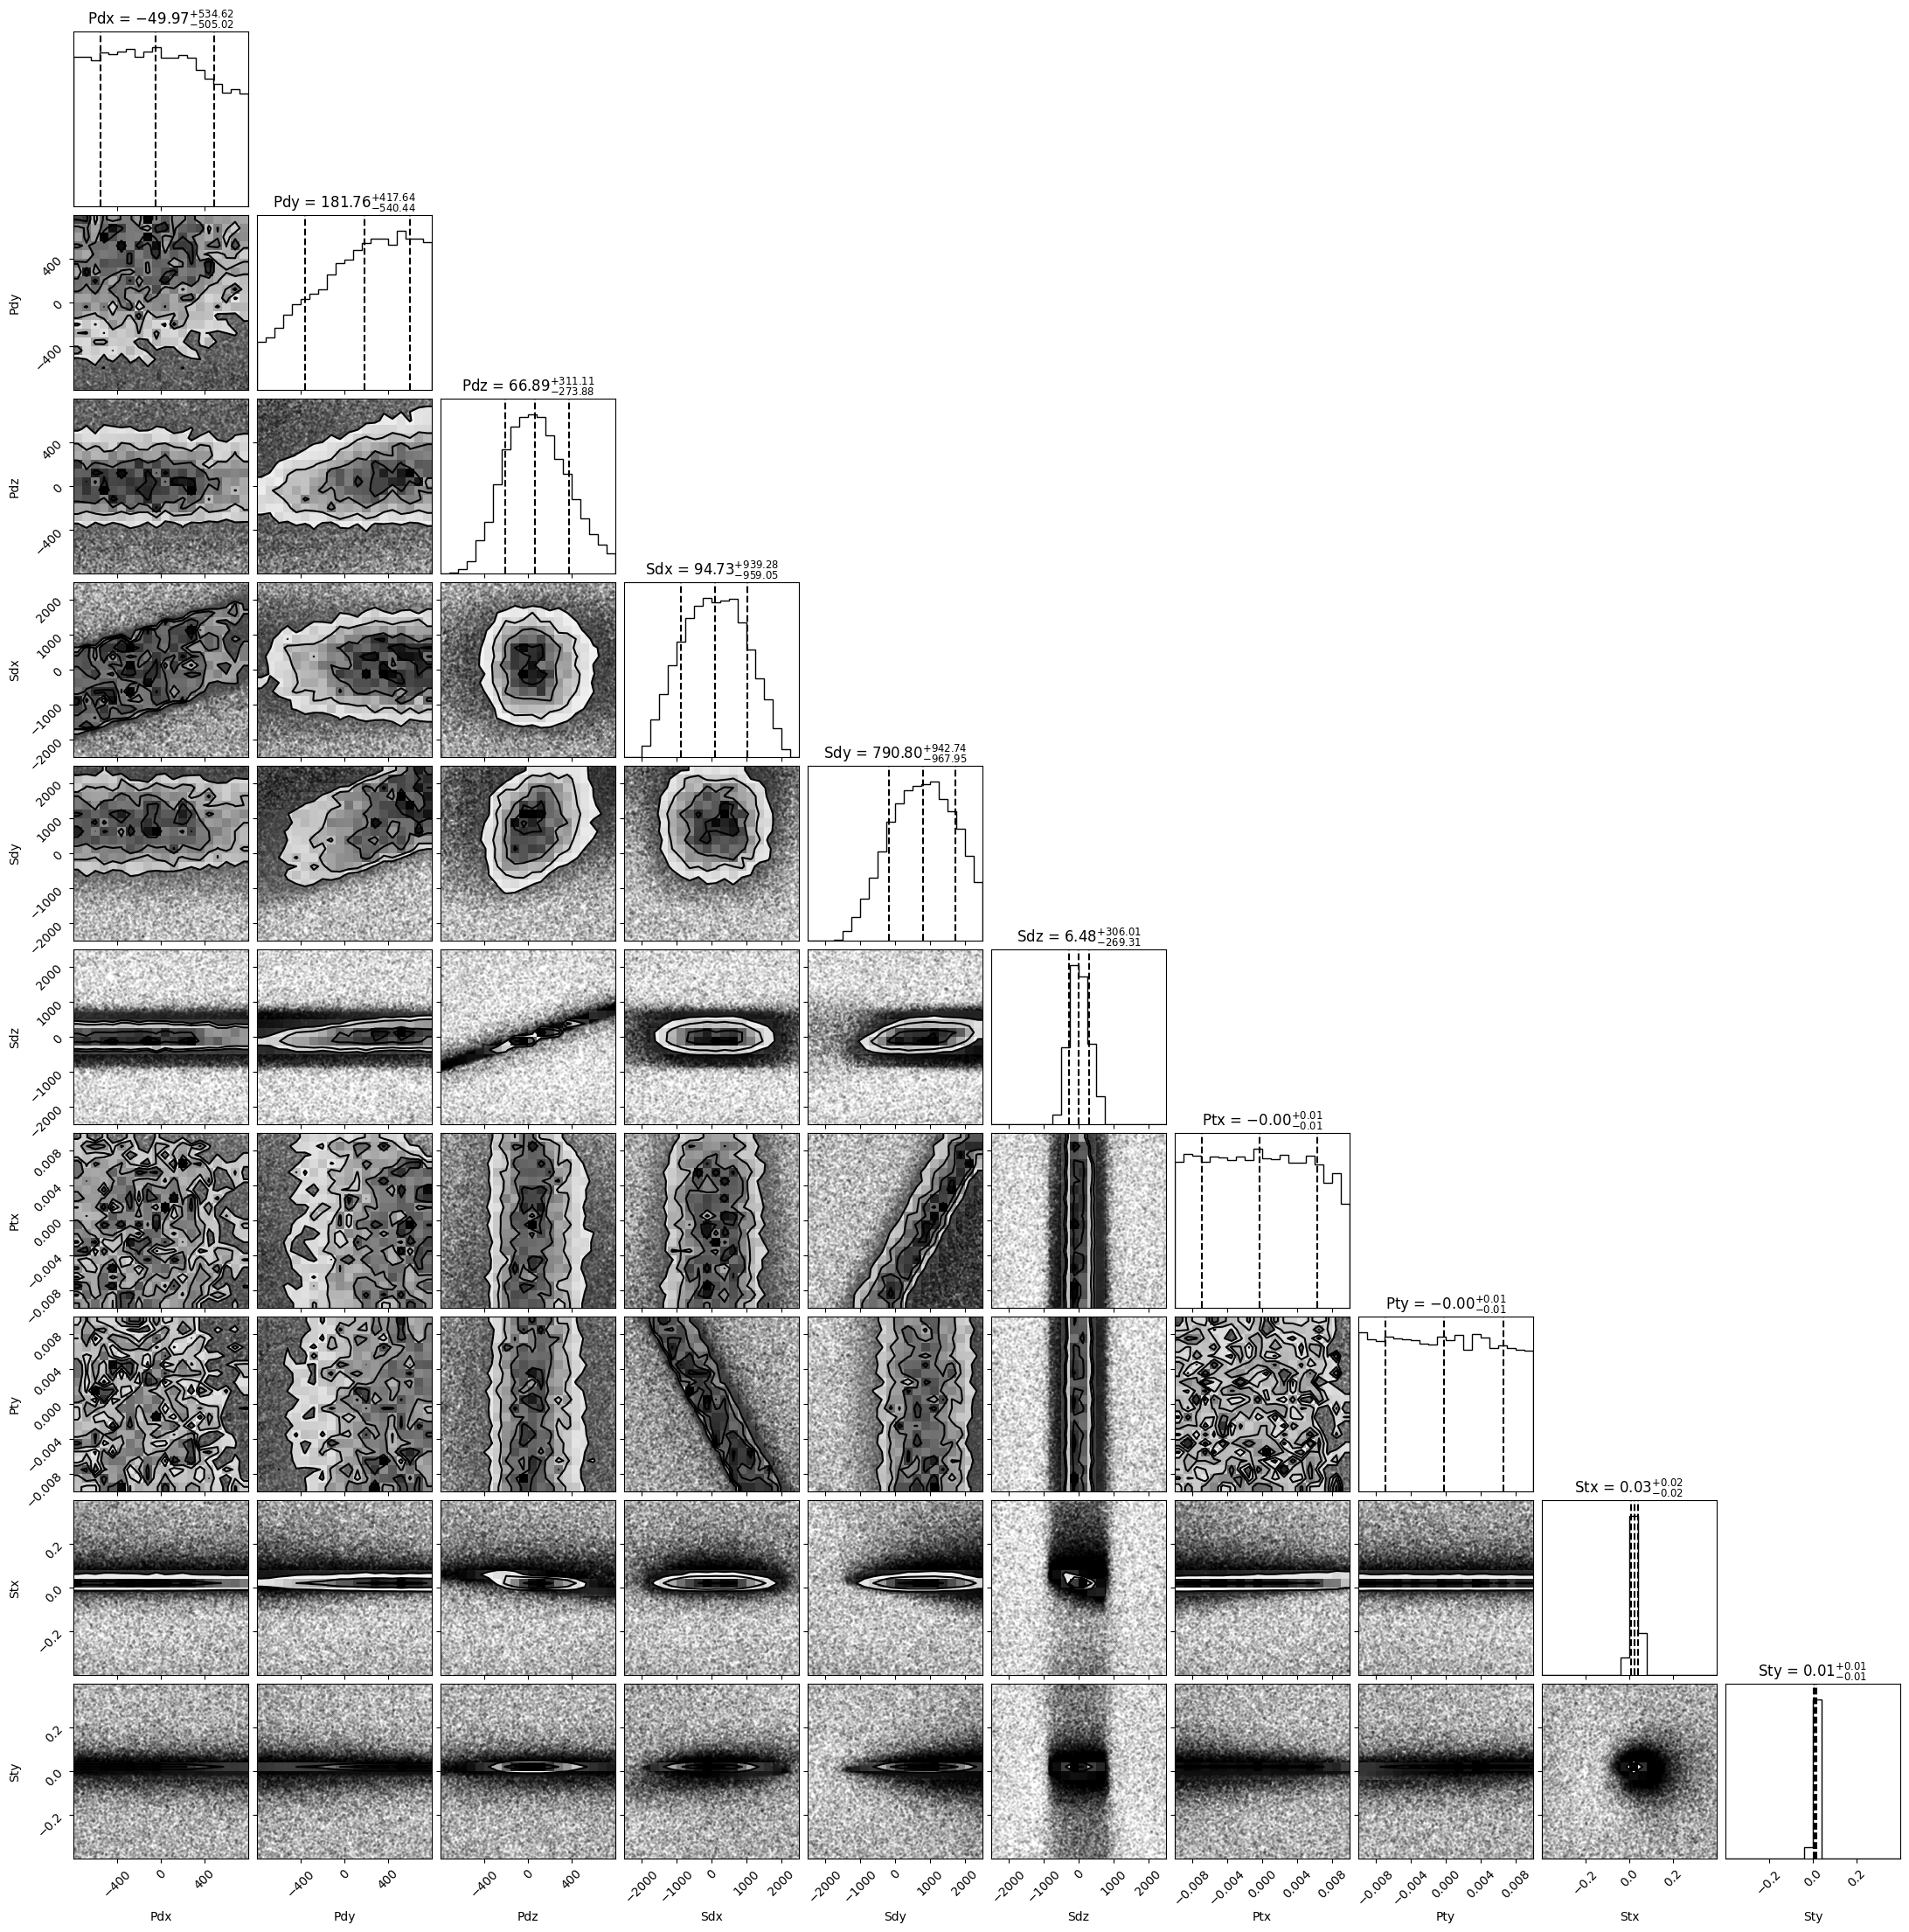
\includegraphics[width=2184\pxu]{../figures/pearltilus.png}};
  % Tint each panel by the kind of pair it shows; multiply keeps the
  % plotted data dark while the white background takes the colour.
  \begin{scope}[blend mode=multiply]
    \fill[prim!22] (84,1974) rectangle (284,2174);
    \fill[prim!22] (84,1764) rectangle (284,1964);
    \fill[prim!22] (294,1764) rectangle (494,1964);
    \fill[prim!22] (84,1554) rectangle (284,1754);
    \fill[prim!22] (294,1554) rectangle (494,1754);
    \fill[prim!22] (504,1554) rectangle (704,1754);
    \fill[cross!22] (84,1344) rectangle (284,1544);
    \fill[cross!22] (294,1344) rectangle (494,1544);
    \fill[cross!22] (504,1344) rectangle (704,1544);
    \fill[sec!12] (714,1344) rectangle (914,1544);
    \fill[cross!22] (84,1134) rectangle (284,1334);
    \fill[cross!22] (294,1134) rectangle (494,1334);
    \fill[cross!22] (504,1134) rectangle (704,1334);
    \fill[sec!12] (714,1134) rectangle (914,1334);
    \fill[sec!12] (924,1134) rectangle (1124,1334);
    \fill[cross!22] (84,924) rectangle (284,1124);
    \fill[cross!22] (294,924) rectangle (494,1124);
    \fill[cross!22] (504,924) rectangle (704,1124);
    \fill[sec!12] (714,924) rectangle (914,1124);
    \fill[sec!12] (924,924) rectangle (1124,1124);
    \fill[sec!12] (1134,924) rectangle (1334,1124);
    \fill[prim!22] (84,714) rectangle (284,914);
    \fill[prim!22] (294,714) rectangle (494,914);
    \fill[prim!22] (504,714) rectangle (704,914);
    \fill[cross!22] (714,714) rectangle (914,914);
    \fill[cross!22] (924,714) rectangle (1124,914);
    \fill[cross!22] (1134,714) rectangle (1334,914);
    \fill[prim!22] (1344,714) rectangle (1544,914);
    \fill[prim!22] (84,504) rectangle (284,704);
    \fill[prim!22] (294,504) rectangle (494,704);
    \fill[prim!22] (504,504) rectangle (704,704);
    \fill[cross!22] (714,504) rectangle (914,704);
    \fill[cross!22] (924,504) rectangle (1124,704);
    \fill[cross!22] (1134,504) rectangle (1334,704);
    \fill[prim!22] (1344,504) rectangle (1544,704);
    \fill[prim!22] (1554,504) rectangle (1754,704);
    \fill[cross!22] (84,294) rectangle (284,494);
    \fill[cross!22] (294,294) rectangle (494,494);
    \fill[cross!22] (504,294) rectangle (704,494);
    \fill[sec!12] (714,294) rectangle (914,494);
    \fill[sec!12] (924,294) rectangle (1124,494);
    \fill[sec!12] (1134,294) rectangle (1334,494);
    \fill[cross!22] (1344,294) rectangle (1544,494);
    \fill[cross!22] (1554,294) rectangle (1754,494);
    \fill[sec!12] (1764,294) rectangle (1964,494);
    \fill[cross!22] (84,84) rectangle (284,284);
    \fill[cross!22] (294,84) rectangle (494,284);
    \fill[cross!22] (504,84) rectangle (704,284);
    \fill[sec!12] (714,84) rectangle (914,284);
    \fill[sec!12] (924,84) rectangle (1124,284);
    \fill[sec!12] (1134,84) rectangle (1334,284);
    \fill[cross!22] (1344,84) rectangle (1544,284);
    \fill[cross!22] (1554,84) rectangle (1754,284);
    \fill[sec!12] (1764,84) rectangle (1964,284);
    \fill[sec!12] (1974,84) rectangle (2174,284);
  \end{scope}
  % Cover the small titles and tick labels (tick marks are kept)
  \fill[white] (84,2177) rectangle (284,2210);
  \fill[white] (294,1967) rectangle (494,2008);
  \fill[white] (504,1757) rectangle (704,1798);
  \fill[white] (714,1547) rectangle (914,1588);
  \fill[white] (924,1337) rectangle (1124,1378);
  \fill[white] (1134,1127) rectangle (1334,1168);
  \fill[white] (1344,917) rectangle (1544,958);
  \fill[white] (1554,707) rectangle (1754,748);
  \fill[white] (1764,497) rectangle (1964,538);
  \fill[white] (1974,287) rectangle (2174,328);
  \fill[white] (0,0) rectangle (2184,75);
  \fill[white] (0,75) rectangle (74,1964);
  % Large parameter names
  \node[font=\fontsize{26}{30}\selectfont] at (184.0,37.5) {$pdx$};
  \node[font=\fontsize{26}{30}\selectfont] at (394.0,37.5) {$pdy$};
  \node[font=\fontsize{26}{30}\selectfont] at (604.0,37.5) {$pdz$};
  \node[font=\fontsize{26}{30}\selectfont] at (814.0,37.5) {$sdx$};
  \node[font=\fontsize{26}{30}\selectfont] at (1024.0,37.5) {$sdy$};
  \node[font=\fontsize{26}{30}\selectfont] at (1234.0,37.5) {$sdz$};
  \node[font=\fontsize{26}{30}\selectfont] at (1444.0,37.5) {$ptx$};
  \node[font=\fontsize{26}{30}\selectfont] at (1654.0,37.5) {$pty$};
  \node[font=\fontsize{26}{30}\selectfont] at (1864.0,37.5) {$stx$};
  \node[font=\fontsize{26}{30}\selectfont] at (2074.0,37.5) {$sty$};
  \node[rotate=90, font=\fontsize{26}{30}\selectfont] at (37,1864.0) {$pdy$};
  \node[rotate=90, font=\fontsize{26}{30}\selectfont] at (37,1654.0) {$pdz$};
  \node[rotate=90, font=\fontsize{26}{30}\selectfont] at (37,1444.0) {$sdx$};
  \node[rotate=90, font=\fontsize{26}{30}\selectfont] at (37,1234.0) {$sdy$};
  \node[rotate=90, font=\fontsize{26}{30}\selectfont] at (37,1024.0) {$sdz$};
  \node[rotate=90, font=\fontsize{26}{30}\selectfont] at (37,814.0) {$ptx$};
  \node[rotate=90, font=\fontsize{26}{30}\selectfont] at (37,604.0) {$pty$};
  \node[rotate=90, font=\fontsize{26}{30}\selectfont] at (37,394.0) {$stx$};
  \node[rotate=90, font=\fontsize{26}{30}\selectfont] at (37,184.0) {$sty$};
  % Strongest primary-secondary degeneracies
  \draw[cross!60!black, line width=5pt] (498,918) rectangle (710,1130);
  \draw[cross!60!black, line width=5pt] (918,708) rectangle (1130,920);
  \draw[cross!60!black, line width=5pt] (708,498) rectangle (920,710);
  % Mirror groups along the columns (x axis)
  \fill[prim] (84,-95) rectangle (704,-15);
  \node[text=white, font=\bfseries\fontsize{20}{24}\selectfont] at (394.0,-55) {PRIMARY};
  \fill[sec] (714,-95) rectangle (1334,-15);
  \node[text=white, font=\bfseries\fontsize{20}{24}\selectfont] at (1024.0,-55) {SECONDARY};
  \fill[prim] (1344,-95) rectangle (1754,-15);
  \node[text=white, font=\bfseries\fontsize{20}{24}\selectfont] at (1549.0,-55) {PRIMARY};
  \fill[sec] (1764,-95) rectangle (2174,-15);
  \node[text=white, font=\bfseries\fontsize{20}{24}\selectfont] at (1969.0,-55) {SECONDARY};
  % Summary table in the empty upper-right triangle
  \node[anchor=north east, inner sep=0pt] (tab) at (2174,2160) {%
    \fontsize{24}{34}\selectfont
    \begin{tabular}{@{}lrll@{}}
      \toprule
      & \bfseries Median & \bfseries 68\% & \bfseries Axis span \\
      \midrule
      \textcolor{prim!85!black}{\bfseries $pdx$} & $-50$ & $^{+535}_{-505}$ & $\pm800\,\mu$m \\
      \textcolor{prim!85!black}{\bfseries $pdy$} & $182$ & $^{+418}_{-540}$ & $\pm800\,\mu$m \\
      \textcolor{prim!85!black}{\bfseries $pdz$} & $67$ & $^{+311}_{-274}$ & $\pm800\,\mu$m \\[3pt]
      \textcolor{sec!85!black}{\bfseries $sdx$} & $95$ & $^{+939}_{-959}$ & $\pm2500\,\mu$m \\
      \textcolor{sec!85!black}{\bfseries $sdy$} & $791$ & $^{+943}_{-968}$ & $\pm2500\,\mu$m \\
      \textcolor{sec!85!black}{\bfseries $sdz$} & $6$ & $^{+306}_{-269}$ & $\pm2500\,\mu$m \\[3pt]
      \textcolor{prim!85!black}{\bfseries $ptx$} & $0.00$ & $\pm0.01$ & $\pm0.01^{\circ}$ \\
      \textcolor{prim!85!black}{\bfseries $pty$} & $0.00$ & $\pm0.01$ & $\pm0.01^{\circ}$ \\[3pt]
      \textcolor{sec!85!black}{\bfseries $stx$} & $0.03$ & $\pm0.02$ & $\pm0.4^{\circ}$ \\
      \textcolor{sec!85!black}{\bfseries $sty$} & $0.01$ & $\pm0.01$ & $\pm0.4^{\circ}$ \\
      \bottomrule
    \end{tabular}};
  % Legend in the empty space to the left of the table (rows 0-1)
  \node[anchor=north east, align=left, font=\fontsize{20}{30}\selectfont,
        fill=white, draw=black!25, inner sep=12pt] at ($(tab.north west)+(-60,0)$) {%
    \textcolor{prim!45}{\rule{1.1em}{0.8em}}\ Primary-mirror pair\\
    \textcolor{sec!25}{\rule{1.1em}{0.8em}}\ Secondary-mirror pair\\
    \textcolor{cross!45}{\rule{1.1em}{0.8em}}\ Primary $\times$ secondary pair\\
    \tikz[baseline=0pt]\draw[cross!60!black, line width=2.5pt] (0,0) rectangle (1.1em,0.8em);\ Strong degeneracy};
\end{tikzpicture}
\end{document}
